\section{Background Theory}
\label{sec:BackgroundTheory}



\subsection{Quantum Mechanics and Information}
\label{sec:SubQMandInfo}

A long acronym entry: \acrlong{QI}.
Author and Year Citations: \citeauthor{Shannon1948} in \citeyear{Shannon1948}.
A definition with mathematical expressions:\\


The conventional system used in \gls{QI} is the \gls{QM} analogue to the Bit:
\begin{defn}\label{def:Q_Reg}
    A \textbf{Quantum Bit} (or \textbf{Qubit}) is a quantum system with basis $B = \{|0\rangle,|1\rangle\}$, whose states $|\psi\rangle$ are therefore of the form
    $$
        |\psi\rangle = \alpha_{0}|0\rangle + \alpha_{1}|1\rangle \, \in \mathcal{H}_{\{0,1\}}, \quad \text{where} \quad
        \alpha_{0}, \alpha_{1} \in \mathbb{C}_{1} \; \big| \; |\alpha_{0}|^{2} + |\alpha_{1}|^{2} = 1
    $$
    A set of qubits is called a \textbf{Quantum Register}; for an $n$-qubit register the state space is then
    $$
        \mathcal{H}_{\{0,1\}^{n}} = \bigotimes_{i=1}^{n} \mathcal{H}_{\{0,1\}} = \mathcal{H}_{\{0,1\}}^{[n]}
    $$
\end{defn}


\begin{equation}\label{eq:CompositeInclusions}
    B^{n} \, \subsetneq \,
    \mathcal{H}_{B}^{n} \, \subsetneq \,
    \mathcal{H}_{B}^{[n]} = \mathcal{H}_{B^{n}}
\end{equation}



\subsection{Visualising Qubit States}
\label{sec:SubVisualStates}

A minipage to show an image beside a column of text:\\

\begin{minipage}{0.5\textwidth} \centering
    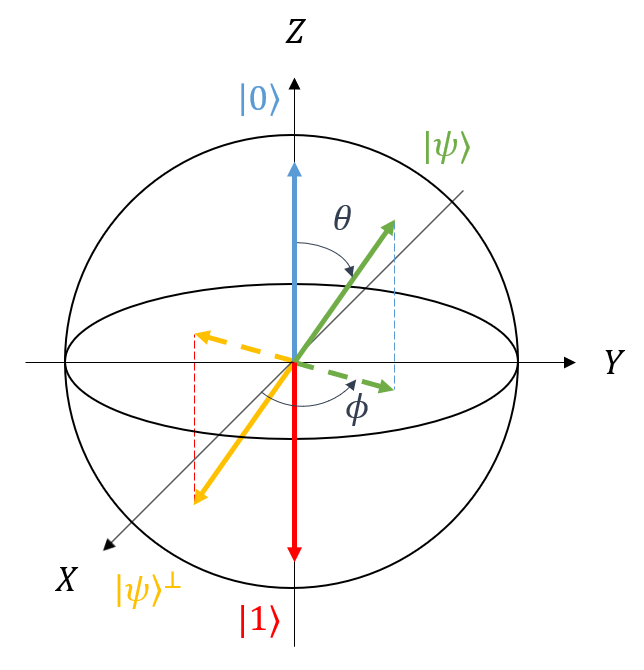
\includegraphics[width=9cm]{BlochSphere}
    \captionof{figure}{\it Bloch Sphere}
    \label{fig:BlochSphere}
\end{minipage}
\begin{minipage}{0.5\textwidth}

Qubit (Pure) States can be visualised on the Bloch Sphere, a unitary sphere in 3D Space, with the standard parametrisation:
$$
    |\psi\rangle = \cos\left(\frac{\theta}{2}\right) |0\rangle + e^{i\phi} \sin\left(\frac{\theta}{2}\right) |1\rangle
$$
Consequently, a Mixture of States can be visualised as a set of vectors on the Bloch Sphere, each associated with a (classical)
probability weighting.\\

A noteworthy feature of the Bloch Sphere is that unlike in standard 3D space, Orthogonality is not given by states $\pi/2$ from
the given one; it is instead given by the (unique) \underline{opposite} state;
it is easy to see that the inner product of opposite states is 0:
\begin{equation}\label{eq:OrthState}
    \alpha |0\rangle + \beta |1\rangle \quad \perp \quad \beta^{*} |0\rangle - \alpha^{*} |1\rangle
\end{equation}

\end{minipage}\\[0.5cm]



\subsection{Entanglement}
\label{sec:SubEntanglement}

An Example:

\begin{exmp}\label{ex:Entanglement}
    In this 3-qubit-system state $|\psi\rangle$, qubits A and B are entangled with each other while in a product state with qubit C:
    \begin{align*}
        |\psi\rangle & = \frac{1}{2\sqrt{2}} (|000\rangle + |010\rangle - |100\rangle + |110\rangle + |001\rangle + |011\rangle - |101\rangle + |111\rangle) \\
                    & = \frac{1}{2\sqrt{2}} (|00\rangle_{AB} + |01\rangle_{AB} - |10\rangle_{AB} + |11\rangle_{AB}) \otimes (|0\rangle_{C} + |1\rangle_{C})
    \end{align*}
    Furthermore, in this case it is not possible to detect the entanglement by just analysing measurement probabilities since they depend on the
    modulus of coefficients, making them equal to those for the state with no $-$ signs.
\end{exmp}


